\documentclass[11pt]{article}
\usepackage{geometry}
\geometry{margin=1in}
\usepackage{booktabs}
\usepackage{array}
\usepackage{tabularx}
\usepackage{longtable}
\usepackage{tikz}
\usepackage{float}
\usepackage{enumitem}
\usepackage[colorlinks=true,linkcolor=blue]{hyperref}
\expandafter\def\expandafter\UrlBreaks\expandafter{\UrlBreaks\do\/\do\.\do\-\do\_\do\:\do\#}
\setlength{\emergencystretch}{5em}
\usetikzlibrary{arrows.meta,positioning,shapes.geometric}
\setlist[itemize]{topsep=2pt,itemsep=2pt,parsep=0pt}
\setlist[enumerate]{topsep=2pt,itemsep=2pt,parsep=0pt}

\title{\textbf{Neo Solidity Compiler\\Design Specification}}
\author{R3E Network}
\date{\today}

\begin{document}
\maketitle
\tableofcontents

\section{Scope and Purpose}
This specification defines the design of the Neo Solidity Compiler (\emph{NSC}), a toolchain that ingests Solidity~0.8.x sources, leverages a Yul-centric pipeline, and emits Neo~N3 artifacts (\path{.nef}, \path{.manifest.json}, ABI metadata, and optional debug bundles). The focus is on architectural correctness, subsystem contracts, and quality attributes needed to reach the ``complete, production-ready'' bar stated in the project README. Implementation details (individual algorithms, data-structure internals) are intentionally out-of-scope.

\subsection{Objectives}
\begin{itemize}
    \item Preserve EVM-visible semantics so Solidity code behaves identically on NeoVM when ABI inputs, storage, and events are equivalent.
    \item Provide a deterministic, testable compilation pipeline with explicit stage boundaries to support certification, auditing, and tooling integration.
    \item Capture Neo-specific design requirements: stack discipline, syscall encoding, manifest population, and devpack alignment.
    \item Document quality and validation responsibilities to ensure a consistent standard for future contributions.
\end{itemize}

\section{References and Terminology}

\subsection{Normative References}
\begin{table}[H]
\centering
\caption{Normative reference set}
\begin{tabularx}{\textwidth}{@{}p{0.12\textwidth}p{0.28\textwidth}X@{}}
\toprule
ID & Artifact & Relevance \\
\midrule
R1 & \path{docs/ARCHITECTURE.md} & Defines baseline architecture, pipeline responsibilities, and sequencing for the production-grade toolchain.\\
R2 & \path{compiler.go} & Hosts the authoritative description of driver phases, configuration knobs, and result surfaces.\\
R3 & \path{YUL_TO_NEOVM_COMPILATION_STRATEGY.md} & Provides the strategy for parsing, normalizing, analysing, and emitting NeoVM bytecode from Yul IR.\\
R4 & \path{docs/mapping_lowering_design.md} & Captures the required design for mapping and indexed storage lowering onto Neo storage primitives.\\
R5 & Repository README & Specifies supported toolchain targets, optimization levels, Neo integration targets, and developer-experience requirements.\\
\bottomrule
\end{tabularx}
\end{table}

\subsection{Terminology}
\begin{description}
    \item[Canonical IR] The SSA-like, Neo-annotated intermediate form consumed by semantic analysis, optimisation, and code generation.
    \item[DevPack] The Neo runtime bindings and Solidity helper surface that map Solidity calls to Neo syscalls, permissions, and native contracts.
    \item[Manifest] The JSON artifact that records ABI, permissions, supported standards, and metadata required by Neo CLI and runtime.
    \item[Runtime Manager] The compiler subsystem that links generated bytecode with runtime stubs, applies policy (execution overrides, metadata), and emits NEF/manifest structures.
    \item[Tooling Adapter] Any CLI or IDE integration (Hardhat plugin, Foundry adapter, \texttt{neo-solc}) that feeds sources into the compiler and consumes diagnostics.
\end{description}

\section{System Objectives and Constraints}
\begin{table}[H]
\centering
\caption{Primary objectives, constraints, and associated design responses}
\begin{tabularx}{\textwidth}{@{}p{0.27\textwidth}p{0.33\textwidth}X@{}}
\toprule
Objective / Constraint & Source & Design Response \\
\midrule
Solidity 0.8.x compatibility with ``complete'' language feature coverage. & README Section~``Core Capabilities'' & Integrate \texttt{solang} frontend for syntax \& semantic parity, normalize to canonical IR preserving source mapping, and extend runtime to cover ABI encoding and event emission.\\
Full Neo N3 deployment outputs (\path{.nef}, \path{.manifest.json}) plus debug metadata. & README Section~``Neo N3 Native'' & Artifact Builder stage emits NEF (CRC32, tokens), manifest (permissions, standards) and optional debug bundles tied to \path{CompilationResult.DebugInfo}.\\
Optimization levels \texttt{-O0} through \texttt{-O3} with gas-sensitive passes. & README Section~``Performance \& Optimization'' & Optimization Engine applies ordered pass suites (constant folding, DCE, stack reduction, Neo-specific peepholes) gated by \path{CompilerConfig.OptimizationLevel}.\\
Deterministic diagnostics and metadata for auditing (400+ tests, VM validation). & README ``Security \& Quality'' and R1 Section~``Testing \& Validation'' & Stage-specific error collection (\texttt{ErrorCollector}), structured warnings, and CI matrix requiring unit, integration, and VM regression suites.\\
Rust~1.70+, Neo~N3 3.0+, CLI/Node tooling availability. & README ``Installation'' & Build scripts assume Rust toolchain, dotnet runtime for Neo runtime library, and Node for tooling packages.\\
\bottomrule
\end{tabularx}
\end{table}

\section{Architectural Overview}
The compiler is organized as a sequence of pure, inspectable stages driven by the Go-based orchestration in \path{compiler.go}. Each stage consumes and produces well-defined data structures stored within \texttt{CompilerContext}. Figure~\ref{fig:pipeline} visualizes the nominal flow.

\begin{figure}[H]
\centering
\resizebox{\textwidth}{!}{%
\begin{tikzpicture}[
    node distance=1.6cm,
    stage/.style={draw, rounded corners, minimum width=3.6cm, minimum height=1.1cm, align=center, fill=gray!10},
    arrow/.style={-{Stealth[length=3mm]}, thick}
]
\node[stage] (sol) {Solidity Source};
\node[stage, right=1.8cm of sol] (yul) {Solang / Yul Parser};
\node[stage, right=1.8cm of yul] (norm) {IR Normalizer};
\node[stage, right=1.8cm of norm] (sem) {Semantic Analyzer};
\node[stage, right=1.8cm of sem] (opt) {Optimization Engine};
\node[stage, right=1.8cm of opt] (code) {NeoVM Code Generator};
\node[stage, right=1.8cm of code] (rt) {Runtime Manager \\ \& Artifact Builder};

\draw[arrow] (sol) -- node[above]{Yul IR} (yul);
\draw[arrow] (yul) -- node[above]{AST} (norm);
\draw[arrow] (norm) -- node[above]{Canonical IR} (sem);
\draw[arrow] (sem) -- node[above]{Validated IR} (opt);
\draw[arrow] (opt) -- node[above]{Optimized IR} (code);
\draw[arrow] (code) -- node[above]{Bytecode} (rt);
\draw[arrow] (rt) -- ++(1.7,0) node[stage, right] (art) {NEF, Manifest, Debug, ABI};
\end{tikzpicture}}
\caption{Compiler pipeline overview}
\label{fig:pipeline}
\end{figure}

\subsection{Stage Contracts}
\begin{table}[H]
\centering
\caption{Pipeline stage responsibilities and invariants}
\begin{tabularx}{\textwidth}{@{}p{0.16\textwidth}p{0.34\textwidth}X@{}}
\toprule
Stage & Responsibilities & Invariants / Outputs \\
\midrule
Frontend & Invoke \texttt{solang} or Yul parser, ingest diagnostics, build \texttt{YulAST}. & AST nodes annotated with \texttt{SourcePosition}, metadata includes compiler version and source identifiers.\\
IR Normalizer & Convert Solang/Yul AST to canonical IR with SSA-like temporaries, explicit control flow. & All identifiers bound, control flow reduced to blocks and jumps, metadata retains traceability (R3 \S4).\\
Semantic Analysis & Build symbol/type tables, enforce Solidity and Neo constraints (storage layout, supported widths, mapping support). & \texttt{TypeTable} populated, warnings/errors classified, runtime safety diagnostics recorded.\\
Optimization & Apply ordered pass list conditioned on \texttt{OptimizationLevel}. & No pass mutates IR outside its ownership, change tracking feeds statistics, stack depth metrics stored for codegen.\\
Code Generation & Emit NeoVM opcodes, manage evaluation and alternative stacks, encode syscalls and control transfer. & Instructions annotated with stack-before/after counts (\texttt{InstructionInfo}), label fixups resolved.\\
Runtime Manager & Attach runtime stubs, compute gas estimates, serialize NEF/manifest, optionally create debug info. & Artifact builder ensures NEF CRC32, manifest compliance, debug maps align with \texttt{SourceMap}.\\
\bottomrule
\end{tabularx}
\end{table}

\section{Component Specifications}

\subsection{Frontend Integration}
\begin{itemize}
    \item \textbf{Inputs:} Solidity sources, compiler flags, metadata describing target NeoVM version.
    \item \textbf{Processing:} Calls Solang to parse Solidity into Yul IR, then feeds Yul text into the internal lexer/parser (R2) to construct \texttt{YulAST}. Lexing includes classification of built-ins (arithmetic, memory, storage, control) to support later optimisation heuristics.
    \item \textbf{Outputs:} AST annotated with source file/line references; initial diagnostics from Solang forwarded through \texttt{ErrorCollector}.
    \item \textbf{Dependencies:} Solang crate, \texttt{YulLexer}, \texttt{YulParser}.
    \item \textbf{Quality Gates:} Empty sources forbidden, keyword table alignment validated on initialisation, parser errors halt compilation before normalization.
\end{itemize}

\subsection{Canonical IR and Normalizer}
\begin{itemize}
    \item \textbf{Purpose:} Provide a deterministic IR that normalizes control flow, imposes SSA-style temporaries, expands built-ins, and records explicit stack/memory effects.
    \item \textbf{Key Behaviors:} Pass suite described in R3 \S4 converts for-loops into jump-based loops, rewrites switch statements into cascaded comparisons, and ensures each variable assignment produces a unique identifier.
    \item \textbf{Metadata:} Maintains source-to-node mapping for downstream debug info.
    \item \textbf{Interface:} \path{Normalizer.Normalize(ast)} returns IR graph or emits normalization errors categorized by phase.
\end{itemize}

\subsection{Semantic Analysis}
\begin{itemize}
    \item \textbf{Scope:} Symbol table construction, type checking, storage layout verification, runtime safety diagnostics (re-entrancy, permission hints per R1).
    \item \textbf{Responsibilities:} Validate mappings (per R4), enforce Neo-supported numeric widths and storage annotations, build metadata for ABI generation (events, functions, state variables).
    \item \textbf{Outputs:} \texttt{analysisResult} containing warnings, errors, and typed IR. Feeds into \path{CompilationResult.Warnings}.
    \item \textbf{Failure Modes:} Missing symbols, unsupported types, invalid storage qualifiers; all must be reported with line/column metadata.
\end{itemize}

\subsection{Optimization Engine}
\begin{itemize}
    \item \textbf{Configuration:} Driven by \path{CompilerConfig.OptimizationLevel}, enabling passes cumulatively from \texttt{-O0} (none) to \texttt{-O3} (all).
    \item \textbf{Pass Library:} Constant folding/propagation; dead code elimination; bounded inlining; stack height reduction; NeoVM-specific peepholes (merge PUSH sequences, syscall hoisting); optional bounds-check insertion when \texttt{EnableBoundsChecking} is true.
    \item \textbf{Accounting:} Each pass records change statistics into the\\
    CompilationStats.\allowbreak OptimizationsPassed counter; the pass manager records before/after IR snapshots for debugging.
    \item \textbf{Constraints:} Passes must preserve semantic equivalence, keep stack effect annotations valid, and honor max stack depth budget.
\end{itemize}

\subsection{NeoVM Code Generator}
\begin{itemize}
\item \textbf{Responsibilities:} Lower canonical IR instructions to NeoVM opcodes (\path{emit_ir_function}, \path{emit_serialize_key}, etc.), allocate locals/arguments via \texttt{INITSLOT}, and encode syscalls with proper interop IDs (storage, crypto, runtime).
    \item \textbf{Stack Discipline:} Maintains explicit stack-before/after counts stored in \texttt{InstructionInfo}; enforces max depth (\path{CompilerConfig.MaxStackDepth}).
    \item \textbf{Control Flow:} All jumps resolved via label fixups; structured exception regions inserted when runtime metadata demands it.
    \item \textbf{Storage Access:} Mapping lowering follows R4 requirements (key serialization, SHA256 hashing, context management) and uses helper routines to ensure consistent key derivation.
\end{itemize}

\subsection{Runtime Manager and Artifact Builder}
\begin{itemize}
    \item \textbf{Runtime Integration:} Links generated bytecode with runtime support (ABI decoder, dispatcher), injects metadata (method table, events), and applies execution overrides via \path{NeoRuntime::execute_with_overrides}.
    \item \textbf{Artifact Generation:} Produces NEF with method tokens and CRC32 checksum, manifest with ABI/permissions/supported standards, ABI JSON for developer tooling, and optional debug bundles (\texttt{DebugInformation}).
    \item \textbf{Policy Hooks:} Applies gas estimates, ensures features flags (storage, dynamic invoke) align with compiled code, and ensures \texttt{CallFlags} usage matches manifest permissions.
\end{itemize}

\subsection{Tooling Surfaces}
\begin{itemize}
    \item \textbf{CLI (\texttt{neo-solc}):} Accepts Sol sources, emits outputs, exposes flags for optimizations, debug info, artifact selection.
    \item \textbf{Hardhat / Foundry Adapters:} Wrap CLI invocation, collect \path{compile_summary.csv}, and map Neo diagnostics to IDE annotations.
    \item \textbf{Debugging Support:} Source maps, function/variable maps for breakpoints (per \texttt{DebugInformation}).
\end{itemize}

\subsection{Hardhat Integration Example}
\begin{small}
\begin{verbatim}
// hardhat.config.js
module.exports = {
  solidity: "0.8.19",
  networks: {
    neo: {
      url: "http://localhost:50012",
      compiler: {
        path: "target/release/neo-solc",
        options: ["-O2", "--debug"]
      }
    }
  },
  neoSolidity: {
    outputDir: "build/neo",
    formats: ["nef", "manifest", "abi"]
  }
};
\end{verbatim}
\end{small}
\noindent Hardhat tasks invoke \texttt{neo-solc} with project-specific options, then copy NEF/manifest outputs into deployment scripts.

\subsection{Foundry Integration Notes}
\begin{itemize}
    \item Configure \texttt{foundry.toml} to point compiler commands at \texttt{neo-solc} for specific profiles. Custom build scripts invoke the CLI for each Solidity contract and capture NEF/manifest outputs in \path{out/neo}.
    \item Foundry tests can execute NEF artifacts via a Neo VM runner (e.g., hooking \texttt{scripts/run_vm_tests.sh}) to compare EVM vs Neo results for parity testing.
    \item Diagnostics emitted by the compiler are converted into Foundry-readable JSON so the IDE surfaces line/column errors in Solidity files.
\end{itemize}

\subsection{DevPack Interface Summary}
\begin{table}[H]
\centering
\caption{Key devpack entry points}
\begin{tabularx}{\textwidth}{@{}p{0.22\textwidth}p{0.2\textwidth}X@{}}
\toprule
Module & Interface & Usage in Compiler \\
\midrule
\texttt{System.Storage} & \texttt{GetContext}, \texttt{Get}, \texttt{Put} & Storage lowering uses these syscalls for state access, ensuring context is fetched once per function when possible.\\
\texttt{System.Runtime} & \texttt{Notify}, \texttt{Log}, \texttt{GetCallingScriptHash} & Event emission, logging, and caller resolution (`msg.sender` semantics).\\
\texttt{System.Contract} & \texttt{Call}, \texttt{CallEx} & Backing for external Solidity calls when mapping to native contracts.\\
\texttt{System.Crypto} & \texttt{SHA256}, \texttt{RIPEMD160} & Mapping key hashing, signature checks, cryptographic helpers.\\
\texttt{System.Blockchain} & \texttt{GetHeight}, \texttt{GetHeader} & Implements Solidity environmental opcodes (block number, timestamp) when ExecutionOverrides are not provided.\\
\bottomrule
\end{tabularx}
\end{table}

\subsection{DevPack API Details}
\begin{table}[H]
\centering
\caption{Storage and Runtime helpers}
\begin{tabularx}{\textwidth}{@{}p{0.24\textwidth}p{0.18\textwidth}X@{}}
\toprule
Module & Function & Notes \\
\midrule
\texttt{System.Storage} & \texttt{GetContext}/\texttt{PutContext} & Context retrieval cached per function when possible; required for all storage reads/writes.\\
\texttt{System.Storage} & \texttt{Get} & Returns byte arrays; compiler inserts deserialization stubs based on IR type.\\
\texttt{System.Storage} & \texttt{Put} & Accepts byte arrays; compiler serializes integers/structs before storing.\\
\texttt{System.Runtime} & \texttt{Notify} & Event emission; compiler builds topic array + ABI-encoded payload.\\
\texttt{System.Runtime} & \texttt{Trace}/\texttt{Log} & Optional instrumentation hooks described in logging section.\\
\texttt{System.Runtime} & \texttt{GetCallingScriptHash} & Used to implement \texttt{msg.sender}.\\
\texttt{System.Crypto} & \texttt{SHA256} & Mapping slot hashing and other cryptographic needs.\\
\texttt{System.Blockchain} & \texttt{GetHeight}, \texttt{GetHeader} & Provide block metadata when ExecutionOverrides absent.\\
\bottomrule
\end{tabularx}
\end{table}

\begin{table}[H]
\centering
\caption{Native contract wrappers}
\begin{tabularx}{\textwidth}{@{}p{0.22\textwidth}p{0.2\textwidth}X@{}}
\toprule
Wrapper & Functionality & Manifest Implications \\
\midrule
PolicyContract & Access to policy contracts (gas price, fee settings) & Requires manifest permission for policy hash; compiler must detect usage and add permission entries.\\
OracleContract & Query oracle results & Permissions include oracle hash; manifest \texttt{features.payable} often true if native oracle requires GAS.\\
ManagementContract & Contract management operations & Restricted to administrative contexts; CLI warns when usage detected without appropriate permissions.\\
LedgerContract & Block/transaction info & Typically read-only; safe flag remains true.\\
\bottomrule
\end{tabularx}
\end{table}


\section{End-to-End Compilation Detail}

\subsection{Solidity Source to Canonical IR}
\begin{enumerate}
    \item \textbf{Solidity Intake:} \texttt{solang} parses Solidity~0.8.x units, applies Solidity semantic rules, and emits Yul-compatible IR plus inline diagnostics. Source maps, type metadata, and modifier contexts are persisted for later mapping into Neo debug info.
    \item \textbf{Yul Parsing:} The internal lexer/parser (\path{YulLexer}, \path{YulParser}) tokenizes Yul IR, classifies built-ins by category, and constructs \texttt{YulAST}. Each AST node records \texttt{SourcePosition} and result-type hints so subsequent passes can reason about evaluation stack effects.
    \item \textbf{Canonicalization:} The normalizer applies the rules captured in R3: convert loops into explicit jump blocks; force SSA-style temporaries; expand complex built-ins (e.g., \texttt{keccak256}) into guardable helper nodes; express control flow exclusively through labeled blocks with deterministic predecessors. During this phase, inline assembly fragments are rejected unless expressible via supported Yul primitives, ensuring deterministic lowering.
    \item \textbf{Semantic Decoration:} The semantic analyzer enriches IR with type ids, storage locations, and binding information. State variables gain explicit storage slots (hashed identifiers, bit widths), while function signatures gain ABI ordinals derived from Solidity selectors. Diagnostics emitted here block compilation if storage layout, inheritance, or modifier resolution fails.
\end{enumerate}

\subsection{Yul-to-NeoVM Conversion Rules}
\paragraph{General Conventions}
\begin{itemize}
    \item Evaluation stack order follows NeoVM semantics (right-most operand on top). Prior to emitting an opcode, the code generator rewrites Yul argument order where necessary so that the stack shape matches the Neo instruction contract. Temporary stack height adjustments rely on \texttt{SWAP}, \texttt{ROT}, and \texttt{DROP} sequences with bounds tracked against \texttt{MaxStackDepth}.
    \item Each NeoVM method starts by reserving locals with \texttt{INITSLOT} using counts derived from IR liveness analysis. Function return values are pushed onto the stack immediately before emitting \texttt{RET}; multi-return sequences follow the ABI order established in the IR metadata.
    \item Branch constructs materialize as labeled blocks. The generator emits placeholders for jump offsets and resolves them after the full method body has been encoded, ensuring canonical byte offsets for manifest/debug metadata.
    \item Syscalls are encoded with their interop ids, pulled from the devpack metadata. The generator centralizes syscall emission so that audit trails can map IR instructions to their concrete \texttt{SYSCALL} operands.
\end{itemize}

\begin{table}[H]
\centering
\caption{Representative Yul~\textrightarrow~NeoVM opcode mapping}
\begin{tabularx}{\textwidth}{@{}p{0.2\textwidth}p{0.33\textwidth}X@{}}
\toprule
Yul Construct & Stack Convention & NeoVM Emission Pattern \\
\midrule
\texttt{add(a,b)} & Push \(b\) then \(a\); result replaces both & \texttt{ADD}. Overflow behavior inherits NeoVM big-int arithmetic; if Solidity semantics require mod-\(2^{256}\), truncation logic inserts \texttt{MOD} with constant modulus.\\
\texttt{mul(a,b)}, \texttt{sub(a,b)} & Same operand ordering as \texttt{add}. & Direct \texttt{MUL}, \texttt{SUB}. Signed variants (\texttt{sdiv}, \texttt{smod}) wrap operands with sign-normalization helpers before emitting \texttt{DIV}/\texttt{MOD}.\\
Comparison (\texttt{lt}, \texttt{gt}, \texttt{eq}) & Evaluates operands, leaves boolean (0/1). & Emits corresponding Neo instructions; signed comparisons insert \texttt{SIGN} normalization.\\
Bitwise (\texttt{and}, \texttt{or}, \texttt{xor}, shifts) & Operands aligned to stack order; shift counts normalized to big-endian. & Uses NeoVM bitwise opcodes; \texttt{shl}/\texttt{shr} translate to \texttt{SHL}/\texttt{SHR}; arithmetic right-shift uses helper that inspects sign bit.\\
\texttt{mload}/\texttt{mstore} & Memory abstraction backed by runtime-managed byte arrays. & Resolves to calls into the runtime memory manager: compute base pointer, call \texttt{System.Runtime.Serialize} or helper stubs, and use \texttt{PICKITEM}/\texttt{SETITEM} to manipulate backing arrays.\\
\texttt{sload}/\texttt{sstore} & Requires slot hash on stack, value for store. & Delegated to storage helpers: push storage context (\texttt{System.Storage.GetContext}), prepare slot byte array, call \texttt{System.Storage.Get}/\texttt{Put}. Mapping keys follow Section~\ref{sec:mapping-detail}.\\
Control flow (\texttt{if}, \texttt{switch}, \texttt{for}) & Conditions evaluated to boolean on stack. & Emit \texttt{JMPIF}/\texttt{JMPIFNOT} plus labels. \texttt{switch} cascades comparisons with duplicated selector values and uses fall-through default blocks (mirroring the pseudo-code in R3~\S5.3).\\
Function call \texttt{f(a,b)} & Arguments pushed reverse order, return slot reserved. & For internal functions, emit \texttt{CALL} to method offset with proper \texttt{INITSLOT}; for external ABI calls, delegate to runtime dispatcher (ABI decoder pushes arguments, selects target).\\
\texttt{revert}/\texttt{return} & Offsets and lengths follow ABI spec. & Use runtime helpers to format return buffers, then emit \texttt{ABORT} or \texttt{RET} with data pointer per ABI encoding rules.\\
\texttt{log{i}} & Topics/data packed on stack. & Call \texttt{System.Runtime.Notify} via devpack wrappers, ensuring topic ordering mirrors Solidity event ABI.\\
\bottomrule
\end{tabularx}
\end{table}

\paragraph{Specific Conversion Rules}
\begin{enumerate}
    \item \textbf{ABI Dispatcher:} Constructor and runtime objects from Yul translate into separate NeoVM entry points. The dispatcher inspects the first 4 bytes of the calldata-equivalent buffer (Neo invocation arguments) and routes to the method offset table. Unknown selectors trigger the standard Solidity revert pattern.
    \item \textbf{Memory Model:} Solidity memory abstractions map onto NeoVM arrays managed by the runtime. \texttt{calldatacopy}, \texttt{returndatacopy}, and ABI encode/decode routines call into runtime helpers that perform bounds checking and convert between little-endian Solidity expectations and Neo big-endian integers.
    \item \textbf{Error Handling:} Solidity \texttt{require}/\texttt{assert} nodes become structured exception blocks. The generator emits predicates, \texttt{JMPIFNOT} gates, and a revert stub that encodes error selectors in ABI-compatible format.
    \item \textbf{Stack Safety:} Each IR instruction carries an expected stack delta; the generator uses this metadata to insert spill-to-alt-stack instructions when stack depth approaches \texttt{MaxStackDepth}, ensuring NeoVM never faults due to stack overflow.
    \item \textbf{Gas/Cost Hints:} While NeoVM gas differs from EVM gas, the generator annotates blocks with syscall counts and arithmetic complexity so the Runtime Manager can compute gross gas estimates stored inside \texttt{CompilationStats}.
\end{enumerate}

\subsection{Opcode Category Mapping}
\begin{table}[H]
\centering
\caption{Category-level mapping reference}
\begin{tabularx}{\textwidth}{@{}p{0.18\textwidth}p{0.3\textwidth}X@{}}
\toprule
Yul Category & Representative Operations & NeoVM Implementation Notes \\
\midrule
Arithmetic & \texttt{add}, \texttt{sub}, \texttt{mul}, \texttt{exp}, \texttt{addmod}, \texttt{mulmod} & Direct opcode emission with optional normalization. Modular variants expand to exponentiation plus \texttt{MOD}. Exponentiation uses \texttt{POW} helper built atop repeated squaring macros owing to NeoVM lacking native exponent opcode.\\
Comparison \& Boolean & \texttt{lt}, \texttt{gt}, \texttt{slt}, \texttt{eq}, \texttt{iszero} & Signed variants translate into sequences that inspect sign bit via \texttt{SIGN} and adjust operands before \texttt{LT}/\texttt{GT}. Boolean negation is \texttt{NOT} applied to 0/1 representation.\\
Bitwise & \texttt{and}, \texttt{or}, \texttt{xor}, \texttt{byte}, \texttt{shl}, \texttt{shr}, \texttt{sar} & Byte extraction implemented using \texttt{PICKITEM} on byte arrays returned by runtime serialization. Arithmetic shift right inserts sign-extension guard around \texttt{SHR}.\\
Memory & \texttt{mload}, \texttt{mstore}, \texttt{mstore8}, \texttt{msize}, \texttt{calldatacopy} & Provided via runtime-managed byte arrays. \texttt{calldatacopy} becomes a runtime call that slices the invocation argument buffer using \texttt{SUBSTR} and writes into contract-managed memory arrays.\\
Storage & \texttt{sload}, \texttt{sstore}, mapping/address ops & Emit \texttt{System.Storage.GetContext} followed by key hashing and \texttt{System.Storage.Get/Put}. Nested mappings rely on the slot-derivation helpers described in Section~\ref{sec:mapping-detail}.\\
Environment & \texttt{gas}, \texttt{timestamp}, \texttt{caller}, \texttt{origin}, \texttt{blockhash} & Bridge to runtime-latched metadata or Neo syscalls (\texttt{System.Blockchain.GetTimestamp}, etc.). When the target attribute is not directly available (e.g., \texttt{gasprice}), shim functions return ABI-compatible placeholders documented in runtime policy.\\
Control Flow & \texttt{if}, \texttt{switch}, \texttt{for}, \texttt{return}, \texttt{revert} & Lower to canonical jump graphs. \texttt{return} uses runtime-managed ABI encoder; \texttt{revert} emits error-selector packaging and jumps to a shared revert stub that aborts execution with encoded data.\\
External Calls & \texttt{call}, \texttt{delegatecall}, \texttt{staticcall} & Neo lacks EVM-style calls, so runtime stubs convert these operations into native-contract invocations or cross-contract dynamic invoke sequences, setting \texttt{CallFlags} according to op semantics (e.g., \texttt{delegatecall} forbids state writes).\\
Events & \texttt{log0}--\texttt{log4} & Map to \texttt{System.Runtime.Notify}, constructing an array of topics and the ABI-encoded data payload. Indexed parameters become topics, matching Solidity's event encoding rules.\\
\bottomrule
\end{tabularx}
\end{table}

\subsection{Lowering Algorithms (Pseudo-code)}
\paragraph{Mapping Load}
\begin{verbatim}
procedure emit_load_mapping(state_index, key_types):
    # stack: [... outer_key, inner_key]
    for key_type in key_types (outermost -> innermost):
        emit_serialize_key(key_type)   # consumes key, pushes canonical bytes
        push slot_hash[state_index]    # 32-byte base slot (first iteration)
        SWAP; CAT                      # concatenate key || slot
        SYSCALL System.Crypto.SHA256   # new slot on stack
    SYSCALL System.Storage.GetContext
    SWAP                              # ensure stack = [context, slot]
    SYSCALL System.Storage.Get        # leaves value
\end{verbatim}

\paragraph{Conditional Lowering}
\begin{verbatim}
procedure lower_if(condition_block, true_block):
    emit evaluate(condition_block)        # leaves boolean on stack
    create label skip_label
    JMPIFNOT skip_label
    emit block(true_block)
    place label skip_label
\end{verbatim}

\paragraph{Switch Lowering}
\begin{verbatim}
procedure lower_switch(expr, cases, default_block):
    emit evaluate(expr)
    DUP
    for case in cases:
        DUP
        PUSH case.value
        EQUAL
        JMPIF case.label
    DROP
    JMP default_label
label blocks emit bodies accordingly
\end{verbatim}

\paragraph{ABI Dispatcher Skeleton}
\begin{verbatim}
procedure dispatcher():
    selector := decode_first_4_bytes(invocation_args)
    switch selector:
        case HASH("transfer(address,uint256)"):
            route_to transfer_impl
        case HASH("balanceOf(address)"):
            route_to balance_impl
        default:
            revert_with_error("Unknown selector")
\end{verbatim}

\subsection{NEF Assembly Workflow}
\begin{enumerate}
    \item \textbf{Method Table Construction:} Each callable entry (public functions, event handlers, static constructors) becomes a method token entry. The compiler records name, parameter count, return count, and instruction pointer offset.
    \item \textbf{Script Buffer Finalization:} After codegen resolves jumps, the byte vector is frozen. Debug metadata (source map, instruction map) stores final offsets so the NEF can point back to Solidity lines.
    \item \textbf{Checksum and Header:} The NEF header embeds compiler information, script length, and checksum. The compiler computes CRC32 over the serialized script and inserts it into the header, matching Neo's validation requirements.
    \item \textbf{Token Serialization:} Method tokens, ABI descriptions, and additional data (e.g., storage ref counters) serialize into the NEF structure per Neo's specification. Optional \texttt{nef.debug.json} is generated in parallel when debug info is enabled.
    \item \textbf{Validation Pass:} Before returning artifacts, the Runtime Manager re-parses the NEF buffer to ensure it meets NeoVM constraints (no unresolved jumps, method offsets within range, CRC match). Failures at this stage are surfaced as Runtime Integration errors.
\end{enumerate}

\subsection{Manifest Generation Workflow}
\begin{enumerate}
    \item \textbf{ABI Extraction:} Symbol tables provide function names, parameter types, visibility, and event topics. Functions become manifest \texttt{methods} entries with offsets and safe parameter metadata; events become \texttt{events} entries with indexed flag information mirroring Solidity's \texttt{indexed} attributes.
    \item \textbf{Permission Derivation:} The code generator records every syscall/native contract reference. The builder groups these references by contract hash or interop service and emits manifest \texttt{permissions}. Devpack annotations determine default groups for runtime services (storage, notifications, crypto).
    \item \textbf{Supported Standards Detection:} Interface conformance (e.g., NEP-11/17/24) is inferred by checking whether contract symbols implement the entire required method set plus event signatures. When matched, the manifest's \texttt{supportedstandards} list receives the corresponding NEP identifier.
    \item \textbf{Features Flags:} The analyzer marks whether storage, dynamic invoke, and payable semantics are used. These booleans map directly to manifest \texttt{features.storage}, \texttt{features.dynamicInvoke}, and \texttt{features.payable}. Payable is enabled when ABI parsing finds functions marked \texttt{payable} or implicit constructors receiving assets.
    \item \textbf{Extra Metadata:} Compilation metadata (compiler version, optimization level, source hash) is attached under the manifest's \texttt{extra} or \texttt{description} fields so downstream tooling can audit builds.
\end{enumerate}

\subsection{NEF Binary Layout}
\begin{table}[H]
\centering
\caption{NEF structural fields}
\begin{tabularx}{\textwidth}{@{}p{0.18\textwidth}p{0.2\textwidth}X@{}}
\toprule
Field & Size (bytes) & Description \\
\midrule
Magic & 4 & Constant header identifying NEF files.\\
Compiler & 32 & ASCII identifier (e.g., ``neo-solidity v1.0.0'').\\
Version & 2 & NEF version supported by target NeoVM.\\
CheckSum & 4 & CRC32 calculated over the entire script payload.\\
Script Length & 2 & Size of the bytecode blob that follows.\\
Script & variable & NeoVM bytecode emitted by code generator.\\
Tokens & variable & Method tokens: name, offset, parameter count.\\
Metadata & variable & Optional debug info pointer, reserve data.\\
\bottomrule
\end{tabularx}
\end{table}

\subsection{NEF Script Hex Example}
\begin{small}
\begin{verbatim}
00000001 6e656f2d736f6c69646974792076312e302e30  # compiler string
0003                                              # NEF version
4f2a6bc1                                          # CRC32
012c                                              # script length (300 bytes)
52 6c 76 68 ...                                   # NeoVM bytecode (truncated)
0200                                              # method token count
077472616e73666572 3402 0100                      # token entry: name, offset, params/returns
...                                               # additional metadata/debug references
\end{verbatim}
\end{small}

\subsection{Manifest Schema Reference}
\begin{table}[H]
\centering
\caption{Manifest key fields}
\begin{tabularx}{\textwidth}{@{}p{0.2\textwidth}p{0.18\textwidth}X@{}}
\toprule
Field & Type & Description \\
\midrule
\texttt{name} & string & Solidity contract name; taken from compilation metadata.\\
\texttt{groups} & array & Future extension (security groups); empty unless specified.\\
\texttt{supportedstandards} & array & List of NEP identifiers automatically inferred.\\
\texttt{abi.methods} & array & Methods with name, parameters, return types, offset.\\
\texttt{abi.events} & array & Events with name, parameters, indexed flags.\\
\texttt{permissions} & array & Each entry references contract hash or wildcard plus allowed methods.\\
\texttt{trusts} & array & Contracts implicitly trusted (rare; enforced via config).\\
\texttt{features.storage} & bool & True when state writes present.\\
\texttt{features.dynamicInvoke} & bool & True if runtime emits dynamic invoke syscalls.\\
\texttt{features.payable} & bool & True if methods accept assets.\\
\texttt{extra} & object/string & Embeds \texttt{CompilationMetadata} snapshot.\\
\bottomrule
\end{tabularx}
\end{table}


\subsection{Mapping Detail Reference}
\label{sec:mapping-detail}
Mapping lowering follows R4 and Section~\ref{sec:mapping-detail} ensures runtime determinism:
\begin{itemize}
    \item Slot hashes are pre-computed at semantic-analysis time using the SHA256 of the state variable name. Nested mappings iterate hashing per key.
    \item Key serialization leverages runtime helpers that convert integers to fixed-width big-endian byte arrays, addresses to 20-byte sequences, and strings to UTF-8 without length prefixes. These helpers return canonical byte arrays consumed by the hashing loop.
    \item Generated code orders keys so the outermost key is on the top of the stack just prior to slot derivation. During hashing, the code alternates between concatenation (\texttt{CAT}) and \texttt{System.Crypto.SHA256}.
    \item Load/store helpers manage stack layout: \texttt{emit\_load\_mapping} expects keys on stack, pushes storage context, and calls \texttt{System.Storage.Get} while preserving evaluation order. Stores ensure values remain on stack until the final \texttt{Put} invocation consumes them.
\end{itemize}

\section{Data and Metadata Structures}

\subsection{Compiler Configuration and Context}
\begin{table}[H]
\centering
\caption{Configuration surface (\texttt{CompilerConfig})}
\renewcommand{\arraystretch}{1.12}
\begin{tabularx}{\textwidth}{@{}p{0.28\textwidth}p{0.18\textwidth}X@{}}
\toprule
Field & Type & Description \\
\midrule
\texttt{OptimizationLevel} & \texttt{int} & Pass suite level (\(0\) to \(3\)); determines aggressive transformations permitted.\\
\texttt{TargetNeoVMVersion} & \texttt{string} & Declares target VM (3.0--3.5+); influences syscall set and manifest compatibility.\\
\texttt{EnableBoundsChecking} & \texttt{bool} & Inserts runtime bounds checks in codegen for memory/array accesses when true.\\
\texttt{EnableDebugInfo} & \texttt{bool} & Enables generation of \texttt{DebugInformation}.\\
\texttt{MaxStackDepth} & \texttt{int} & Upper bound for evaluation stack depth; codegen must enforce.\\
\texttt{MemoryLimit} & \texttt{int64} & Max memory used during compilation (defensive against large contracts).\\
\texttt{CompilerFlags} & \texttt{[]string} & Additional feature toggles, e.g., experimental passes or manifest policies.\\
\bottomrule
\end{tabularx}
\end{table}

\begin{table}[H]
\centering
\caption{Core context and result records}
\renewcommand{\arraystretch}{1.12}
\begin{tabularx}{\textwidth}{@{}p{0.27\textwidth}p{0.25\textwidth}X@{}}
\toprule
Structure & Key Fields & Purpose \\
\midrule
\texttt{CompilerContext} & \texttt{SourceMap}, \texttt{SymbolTable}, \texttt{TypeTable}, \texttt{LabelCounter}, \texttt{ErrorCollector}, \texttt{CompilationMetadata} & Shared state across stages; ensures consistent symbol/type resolution and diagnostic aggregation.\\
\texttt{CompilationResult} & \texttt{Contract}, \texttt{Warnings}, \texttt{Errors}, \texttt{Statistics}, \texttt{DebugInfo} & Final deliverable to tooling; either contains emitted artifacts or records failure causes per phase.\\
\texttt{CompilationMetadata} & \texttt{CompilerVersion}, \texttt{CompilationTime}, \texttt{SourceHash}, \texttt{Statistics} & Audit trail for builds; used in debug bundles and manifest extra metadata.\\
\texttt{DebugInformation} & \texttt{SourceMap}, \texttt{FunctionMap}, \texttt{VariableMap}, \texttt{InstructionMap} & Enables IDEs/debuggers to map bytecode offsets back to source constructs.\\
\bottomrule
\end{tabularx}
\end{table}

\subsection{Diagnostic Contracts}
\begin{itemize}
    \item \textbf{Severity Levels:} Errors (fatal) and warnings (non-fatal) per \texttt{CompilerError} and \texttt{CompilerWarning}.
    \item \textbf{Phase Tagging:} Every diagnostic ties back to the emitting stage (\emph{Parsing}, \emph{Normalization}, \emph{Static Analysis}, etc.) to support stage-by-stage gating and analytics.
    \item \textbf{Traceability:} All diagnostics must carry source locations when available; emitted artifacts maintain \texttt{SourceMap} keyed by bytecode offsets.
\end{itemize}

\section{Control Flow, State Management, and Runtime Coordination}
\subsection{Compiler State Machine}
\begin{longtable}{@{}p{0.17\textwidth}p{0.33\textwidth}p{0.4\textwidth}@{}}
\caption{State transitions}\label{tab:states}\\
\toprule
State & Entry Condition & Exit Condition \\
\midrule
\endfirsthead
\toprule
State & Entry Condition & Exit Condition \\
\midrule
\endhead
Initialized & \texttt{NewYulToNeoCompiler} invoked; context allocated. & Parser consumes first token from source.\\
Parsed & \path{Parser.Parse} succeeded. & \path{Normalizer.Normalize} completes; invalid AST halts pipeline.\\
Normalized & Canonical IR built. & Semantic analyzer validates and populates symbol/type tables.\\
Analyzed & Semantic checks completed; warnings recorded. & Optimization passes applied successfully.\\
Optimized & All enabled passes report success; IR annotated with stack metrics. & Code generator emits bytecode without exceeding stack/memory constraints.\\
Generated & Bytecode exists; instruction metadata built. & Runtime manager attaches runtime artifacts, NEF, manifest.\\
Finalized & Contract artifacts available; debug info optional. & Compilation result returned to caller or CLI for persistence.\\
\bottomrule
\end{longtable}

\subsection{Runtime Layering}
\begin{figure}[H]
\centering
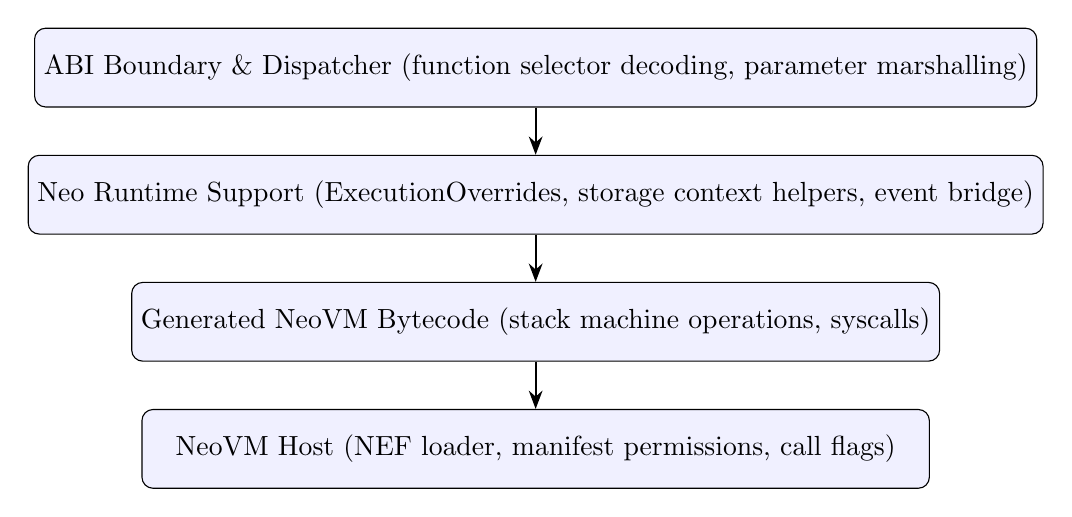
\begin{tikzpicture}[
    layer/.style={draw, rounded corners, minimum width=10cm, minimum height=1cm, align=center, fill=blue!6},
    >=Stealth
]
\node[layer] (abi) {ABI Boundary \& Dispatcher (function selector decoding, parameter marshalling)};
\node[layer, below=0.6cm of abi] (runtime) {Neo Runtime Support (ExecutionOverrides, storage context helpers, event bridge)};
\node[layer, below=0.6cm of runtime] (bytecode) {Generated NeoVM Bytecode (stack machine operations, syscalls)};
\node[layer, below=0.6cm of bytecode] (platform) {NeoVM Host (NEF loader, manifest permissions, call flags)};
\draw[->, thick] (abi) -- (runtime);
\draw[->, thick] (runtime) -- (bytecode);
\draw[->, thick] (bytecode) -- (platform);
\end{tikzpicture}
\caption{Runtime layering and responsibilities}
\label{fig:runtime-layers}
\end{figure}

\subsection{Execution Overrides}
\begin{itemize}
    \item \textbf{Design Intent:} Allow deterministic injection of block height, timestamp, and calling script hash for tests without mutating global runtime state (per README ``Runtime Metadata Overrides'').
    \item \textbf{Mechanism:} \path{NeoRuntime::execute_with_overrides} accepts \texttt{ExecutionOverrides}, executes one invocation, and returns \texttt{ExecutionResult} carrying \texttt{ExecutionMetadata}.
    \item \textbf{Constraints:} Overrides apply to a single execution, clear afterwards, and default to \texttt{RuntimeConfig} otherwise.
\end{itemize}

\section{Optimization and Analysis Strategy}
\begin{table}[H]
\centering
\caption{Optimization pass catalog}
\begin{tabularx}{\textwidth}{@{}p{0.18\textwidth}p{0.22\textwidth}X@{}}
\toprule
Pass & Trigger Level & Notes \\
\midrule
Constant Folding / Propagation & \texttt{-O1}--\texttt{-O3} & Simplifies arithmetic, comparisons, and branches when operands literalized by frontend.\\
Dead Code Elimination & \texttt{-O1}--\texttt{-O3} & Removes unreachable blocks and unused assignments; ensures elimination respects event side-effects.\\
Function Inlining & \texttt{-O2}--\texttt{-O3} & Applies heuristics based on stack depth budget and call frequency; avoids recursion.\\
Stack Height Reduction & \texttt{-O2}--\texttt{-O3} & Peephole rewriting to minimize DUP/SWAP sequences before codegen (R3 \S6.4).\\
Neo-Specific Peepholes & \texttt{-O3} & Merges adjacent \texttt{PUSH} ops, hoists repeated syscall operands, balances alt-stack usage.\\
Bounds Check Injection & Optional flag & Ensures safe memory and array access; complements \texttt{EnableBoundsChecking}.\\
Gas Estimation & Always-on & Tracks syscall/gas usage for reporting; influences manifest \texttt{features}.\\
\bottomrule
\end{tabularx}
\end{table}

\section{Artifact Production and Interfaces}
\subsection{Artifact Catalog}
\begin{table}[H]
\centering
\caption{Generated artifacts and consumers}
\renewcommand{\arraystretch}{1.12}
\begin{tabularx}{\textwidth}{@{}p{0.18\textwidth}p{0.32\textwidth}X@{}}
\toprule
Artifact & Contents & Consumers / Notes \\
\midrule
NEF (\path{*.nef}) & Bytecode, method tokens, checksum. & Neo CLI, NeoExpress, runtime host; must align with target Neo version.\\
Manifest (\path{*.manifest.json}) & ABI signatures, events, permissions, supported standards, \texttt{features}. & Deployment pipelines, policy validators; derived from semantic metadata.\\
ABI JSON & Function/event descriptors for tooling. & Hardhat plugin, Foundry adapter, language servers.\\
Debug Bundle (\path{nef.debug.json}) & Source map, instruction map, variable map. & Debuggers and IDE breakpoints (per README ``Rich Debugging'').\\
Compile Summary (\path{compile_summary.csv}) & Batch compilation outcomes. & CI reporting, regression dashboards (README ``Batch Compilation'').\\
\bottomrule
\end{tabularx}
\end{table}

\subsection{Manifest Construction Rules}
\begin{itemize}
    \item \textbf{ABI:} Derived from symbol tables (functions, events, state variables); honours overload resolution and parameter types.
    \item \textbf{Permissions:} For each syscall/native contract usage discovered during codegen, manifest must include corresponding \texttt{permissions} entries.
    \item \textbf{Supported Standards:} NEP-11/17/24 flags automatically populated when devpack contracts or interfaces detected in sources.
    \item \textbf{Features:} \texttt{storage}, \texttt{dynamicInvoke}, \texttt{payable} toggles computed based on IR analysis and runtime instrumentation.
\end{itemize}

\section{Storage and Mapping Design}
\subsection{Mapping and Indexed Storage Lowering}
The compiler must follow the plan in R4 when lowering mappings and struct-field references:
\begin{enumerate}
\item \textbf{Representation:} Extend IR types with ValueType::Mapping and instructions\\
(\texttt{LoadMapping}, \texttt{StoreMapping}, \texttt{AddressOfMapping}, \texttt{LoadStructField}, \texttt{StoreStructField}).
    \item \textbf{Key Serialization:} Serialize keys using canonical rules (big-endian padded integers, UTF-8 strings, raw bytes for addresses). Keys pushed in reverse order such that the outermost key sits on top of the stack before hashing.
    \item \textbf{Slot Derivation:} For each key, compute \(\mathrm{SHA256}(key\_bytes \Vert slot)\) starting from the pre-computed state-variable slot hash.
    \item \textbf{Syscall Ordering:} After slot derivation, push storage context via\\
    System.Storage.\allowbreak GetContext, reorder stack to match syscall signatures, and invoke\\
    System.Storage.\allowbreak Get or \texttt{Put}.
    \item \textbf{Diagnostics:} Reject unsupported value types, warn when values contain dynamic arrays (future work), and trace stack shapes for debugging.
\end{enumerate}

\subsection{Memory Layout Assumptions}
\begin{itemize}
    \item Persistent state resides in Neo storage, addressed via 32-byte slot hashes.
    \item Evaluation stack hosts temporaries, call arguments, and return slots; alt-stack used sparingly for spills.
    \item Runtime-managed buffers (ABI encoding/decoding) obey Neo serialization routines to remain deterministic across nodes.
\end{itemize}

\subsection{Storage Slot Hashing Diagram}
\begin{figure}[H]
\centering
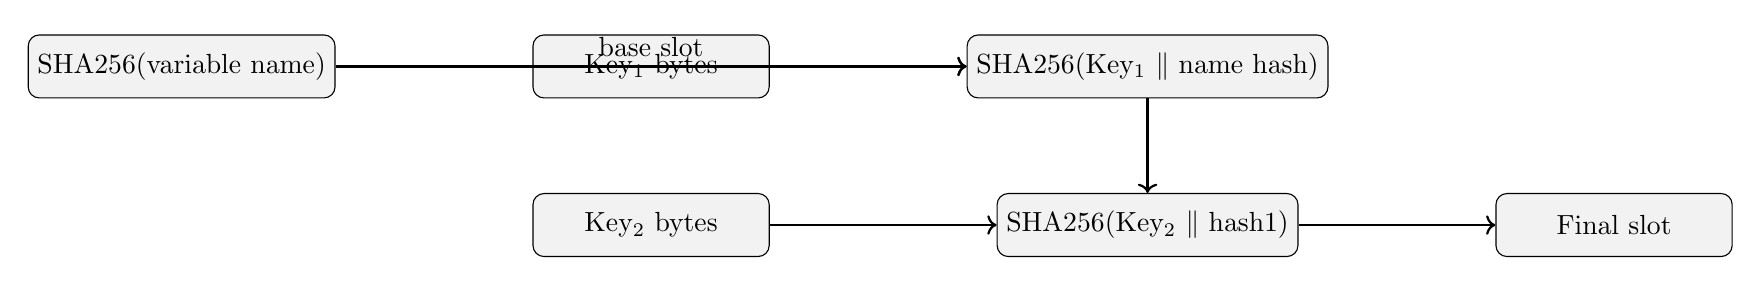
\begin{tikzpicture}[
    node distance=1.6cm,
    slot/.style={draw, rounded corners, minimum width=3cm, minimum height=0.8cm, align=center, fill=gray!10},
    arrow/.style={->, thick}
]
\node[slot] (name) {SHA256(variable name)};
\node[slot, right=2.5cm of name] (key1) {Key\(_1\) bytes};
\node[slot, right=2.5cm of key1] (hash1) {SHA256(Key\(_1\) \(\Vert\) name hash)};
\node[slot, below=1.2cm of key1] (key2) {Key\(_2\) bytes};
\node[slot, below=1.2cm of hash1] (hash2) {SHA256(Key\(_2\) \(\Vert\) hash1)};
\node[slot, right=2.5cm of hash2] (final) {Final slot};
\draw[arrow] (name) -- node[above]{base slot} (hash1);
\draw[arrow] (key1) -- (hash1);
\draw[arrow] (hash1) -- (hash2);
\draw[arrow] (key2) -- (hash2);
\draw[arrow] (hash2) -- (final);
\end{tikzpicture}
\caption{Nested mapping slot derivation}
\label{fig:mapping-hash}
\end{figure}

\section{Diagnostics, Security, and Quality Attributes}
\subsection{Diagnostic Strategy}
\begin{itemize}
    \item \textbf{Phase-specific messaging:} Errors/warnings attach phase tags to support gating (e.g., CLI can stop after parsing warnings if \texttt{--fail-on-warning} is set).
    \item \textbf{Source Mapping:} \texttt{buildSourceMap}, \texttt{buildFunctionMap}, \texttt{buildVariableMap}, and \texttt{buildInstructionMap} ensure every emitted instruction can be traced back to a source region.
    \item \textbf{Logging:} Each driver stage logs start/end markers (see R2 logging statements) for observability.
\end{itemize}

\subsection{Security Considerations}
\begin{itemize}
    \item \textbf{Compiler Security:} Input validation, resource limits (\texttt{MemoryLimit}), and deterministic output guard against compiler-level DoS or inconsistent builds (R3 \S13.1).
    \item \textbf{Runtime Security:} Bounds checking, stack depth monitoring, and call validation (call flags vs manifest) uphold Neo runtime safety expectations (R3 \S13.2).
    \item \textbf{Metadata Integrity:} CRC32 for NEF, manifest hashing, and recorded \texttt{SourceHash} ensure artifact provenance.
\end{itemize}

\subsection{Security Posture and Monitoring}
\begin{itemize}
    \item \textbf{Audit Trail:} Every compilation emits \texttt{CompilationMetadata} (compiler version, source hash, configuration) stored in manifests and debug bundles, enabling auditors to verify the exact toolchain used for deployment.
    \item \textbf{Logging Integration:} Structured logs produced by runtime instrumentation can feed into SIEM systems to monitor contract behavior, detect abnormal storage writes, and correlate revert reasons across deployments.
    \item \textbf{Supply Chain Controls:} Release artifacts (binaries, NEFs, spec PDF) include checksums and signatures. CI enforces reproducible builds by pinning toolchain versions (Rust, Go, dotnet).
    \item \textbf{Monitoring Hooks:} The compiler can emit optional health-check endpoints or telemetry events summarizing compilation errors/warnings, enabling teams to monitor code health across repositories.
    \item \textbf{Audit Readiness:} The spec, manifest metadata, and traceability matrix collectively provide auditors with a single reference covering architecture, testing, and configuration surfaces. Teams are encouraged to keep this spec updated per release.
\end{itemize}

\subsection{Telemetry and Metrics Export}
\begin{itemize}
    \item \textbf{Compilation Metrics:} The CLI can emit metrics (JSON or Prometheus exposition) summarizing \texttt{CompilationStats} (compile time, bytecode size, optimization counts) so build systems can monitor regressions over time.
    \item \textbf{Runtime Metrics:} Instrumentation hooks allow exporting syscall counts, storage operations, and stack depth usage during VM regression tests. These metrics help tune optimization passes and detect abnormal patterns.
    \item \textbf{Environment Compatibility:} The same telemetry endpoints can differentiate between local, TestNet, and MainNet builds by tagging metrics with environment labels derived from \texttt{ExecutionOverrides} or CLI flags.
    \item \textbf{Collection Pipeline:} Metrics are typically written to \path{build/reports/metrics.json} and optionally pushed to monitoring systems. CI jobs archive these reports alongside NEF/manifest artifacts for future analysis.
\end{itemize}

\section{Validation and Compliance}
\subsection{Test Strategy}
\begin{table}[H]
\centering
\caption{Validation layers}
\begin{tabularx}{\textwidth}{@{}p{0.2\textwidth}p{0.25\textwidth}X@{}}
\toprule
Layer & Coverage & Evidence / Tooling \\
\midrule
Unit Tests & Lexer/parser, semantic rules, optimizer passes, mapping lowering helpers. & Rust/Go test suites under \texttt{src}, \texttt{tests}, targeting canonical IR transformations.\\
Integration Tests & Reference contracts (NEP-11/17/24, Uniswap suite) compiled end-to-end. & Batch compilation command (README \S``Batch Compilation'') with \path{compile_summary.csv} showing \(132\) successes baseline.\\
VM Regression & Execute generated NEF in Neo VM runner or NeoExpress, validate observable behavior matches Solidity expectations. & \path{NeoRuntime::execute_with_overrides} harness plus NEP sample manifests.\\
Static/Quality Analysis & Linting (\texttt{cargo fmt}, \texttt{clippy}), code metrics, security scans. & GitHub Actions matrix as described in R1 ``Testing \& Validation''.\\
\bottomrule
\end{tabularx}
\end{table}

\subsection{Test Matrix and Coverage Goals}
\begin{table}[H]
\centering
\caption{Representative contract suite coverage}
\begin{tabularx}{\textwidth}{@{}p{0.24\textwidth}p{0.18\textwidth}X@{}}
\toprule
Suite & Contracts & Purpose \\
\midrule
Core NEP Set & NEP-11, NEP-17, NEP-24 reference implementations & Validates token standards, event emission, mapping storage correctness.\\
Uniswap Reference & 130+ Solidity contracts in \path{uniswap/} & Exercises complex inheritance, libraries, ABI interactions; captures real-world deployment scenarios.\\
Runtime Scenarios & Synthetic contracts covering syscalls, storage edge cases, exception handling & Ensures runtime helpers (ExecutionOverrides, storage hashing) behave correctly.\\
DevPack Examples & Contracts relying on Neo native contracts (oracle, policy, management) & Verifies interop IDs, manifest permissions, and devpack wrappers.\\
\bottomrule
\end{tabularx}
\end{table}

\subsection{Continuous Integration Flow}
\begin{itemize}
    \item \textbf{Static Checks:} \texttt{cargo fmt}, \texttt{clippy}, Go formatters, and TypeScript linting (where applicable) run in parallel jobs.
    \item \textbf{Unit/Integration Tests:} Rust and Go unit tests execute ahead of integration suites. Integration stage compiles the NEP set plus Uniswap suite, persisting \path{compile_summary.csv} artifacts for failure triage.
    \item \textbf{VM Regression:} Selected NEF outputs run inside NeoExpress or the Neo VM runner to assert runtime behavior (deploy + method invocation). Failures break the pipeline and surface logs with bytecode diffs.
    \item \textbf{Artifact Validation:} Generated NEF/manifest pairs undergo schema validation, checksum verification, and manifest-permission sanity checks.
    \item \textbf{Publishing:} On tagged releases, the pipeline packages binaries, attaches NEF/manifest samples, and uploads the refreshed PDF spec as a release artifact for consumer reference.
\end{itemize}

\subsection{CI Artifact Summary}
\begin{table}[H]
\centering
\caption{Uploaded artifacts per pipeline run}
\begin{tabularx}{\textwidth}{@{}p{0.24\textwidth}p{0.18\textwidth}X@{}}
\toprule
Artifact & Location & Purpose \\
\midrule
\path{compile_summary.csv} & \path{build/reports} & Tracks contract compilation outcomes; consumed by dashboards.\\
\path{build/nefs/*.nef} & \path{build/nefs} & Compiled bytecode for inspection or deployment tests.\\
\path{build/manifests/*.manifest.json} & \path{build/manifests} & Manifest outputs paired with NEFs.\\
\path{spec/neo_solidity_compiler_design_spec.pdf} & Release artifacts & Provides the latest formal spec to consumers.\\
\path{logs/*.txt} & \path{build/logs} & Contains integration/VM run logs for failure triage.\\
\bottomrule
\end{tabularx}
\end{table}

\subsection{CI Command Summary}
\begin{table}[H]
\centering
\caption{Key CI commands per stage}
\begin{tabularx}{\textwidth}{@{}p{0.18\textwidth}p{0.24\textwidth}X@{}}
\toprule
Stage & Command & Purpose \\
\midrule
Format/Lint & \texttt{cargo fmt -- --check}, \texttt{cargo clippy}, \texttt{go fmt ./...} & Ensures code style consistency before tests.\\
Unit Tests & \texttt{cargo test --all}, \texttt{go test ./...} & Verifies lexer/parser/codegen helpers and Go runtime pieces.\\
Integration Tests & \texttt{scripts/compile\_nep\_suite.sh}, \texttt{scripts/compile\_uniswap.sh} & Produces NEF/manifest outputs and \path{compile_summary.csv}.\\
VM Regression & \texttt{scripts/run\_vm\_tests.sh} (NeoExpress) & Executes NEFs inside a VM runner, capturing logs.\\
Artifact Packaging & \texttt{scripts/package\_release.sh} & Bundles binaries, NEFs, manifests, and spec PDF for release.\\
\bottomrule
\end{tabularx}
\end{table}

\subsection{Sample CI Pipeline}
\begin{small}
\begin{verbatim}
name: CI
on: [push, pull_request]
jobs:
  build:
    runs-on: ubuntu-latest
    steps:
      - uses: actions/checkout@v4
      - uses: actions/setup-rust@v1
        with: {rust-version: 1.70}
      - run: cargo fmt -- --check
      - run: cargo clippy -- -D warnings
      - run: cargo test --all
      - run: scripts/compile_nep_suite.sh
      - run: scripts/compile_uniswap.sh
      - run: scripts/run_vm_tests.sh
      - name: Upload artifacts
        uses: actions/upload-artifact@v4
        with:
          name: neo-solidity-artifacts
          path: |
            build/nefs
            build/manifests
            build/reports/compile_summary.csv
            spec/neo_solidity_compiler_design_spec.pdf
\end{verbatim}
\end{small}

\subsection{Compile Summary Artifact}
\begin{small}
\begin{verbatim}
contract, result, warnings, errors, elapsed_ms
NEP17.sol, success, 0, 0, 352
UniswapV2Router.sol, success, 1, 0, 812
UniswapV2Pair.sol, success, 0, 0, 644
OracleExample.sol, failure, 0, 1, 115
\end{verbatim}
\end{small}
\noindent CI jobs upload \path{compile_summary.csv} so downstream dashboards can trend success rates and highlight regressions.



\subsection{Traceability Matrix}
\begin{longtable}{@{}p{0.23\textwidth}p{0.27\textwidth}p{0.4\textwidth}@{}}
\caption{Requirement traceability}\label{tab:trace}\\
\toprule
Requirement & Satisfied By & Verification \\
\midrule
\endfirsthead
\toprule
Requirement & Satisfied By & Verification \\
\midrule
\endhead
Solidity feature parity & Frontend + Semantic Analyzer components. & Differential testing vs Solang diagnostics, integration suite results.\\
Neo artifact emission & Runtime Manager + Artifact Builder. & Inspection of NEF/manifest outputs, deployment via Neo CLI.\\
Optimization levels & Optimization Engine configuration. & Unit tests per pass, CLI flag tests, compilation statistics.\\
Debugging support & DebugInformation builders. & IDE integration tests ensuring breakpoints map to instructions.\\
Mapping lowering correctness & Code generator helpers per R4. & Unit tests with NEP-17 storage patterns, VM validation of mapping operations.\\
Runtime metadata overrides & \texttt{ExecutionOverrides} contract in runtime. & Tests invoking \path{execute_with_overrides}, verifying metadata payload.\\
\bottomrule
\end{longtable}

\section{Assumptions and Future Work}
\begin{itemize}
    \item Licensing resolution for Solang remains open (R1 ``Open Questions''); if unresolved, fallback to consuming \texttt{solc} JSON outputs.
    \item Storage layout alignment with Neo key-value model is partially addressed (mappings complete; dynamic arrays scheduled as follow-up).
    \item Gas accounting strategy may evolve as Neo provides more precise estimators.
    \item Debug info format should be reconciled with Neo debugger expectations once specifications are finalized.
\end{itemize}

\subsection{Planned Enhancements}
\begin{itemize}
    \item \textbf{Dynamic Array Lowering:} Extend the mapping/storage infrastructure to cover packed dynamic arrays, including slice operations and bounds-check optimizations.
    \item \textbf{Formal Debug Spec Alignment:} Collaborate with Neo debugger maintainers to lock down the \texttt{nef.debug.json} schema, ensuring IDE tooling can rely on stable contracts.
    \item \textbf{Incremental Compilation:} Investigate caching canonical IR fragments to reduce compile times for iterative development workflows.
    \item \textbf{DevPack API Coverage:} Document and integrate additional native contract wrappers (e.g., oracle, ledger) with exhaustive manifest permission derivation.
    \item \textbf{CI Enhancements:} Add mutation/fuzz testing stages and automated manifest permission linting to catch regressions earlier.
\end{itemize}

\subsection{Cross-Chain Compatibility Considerations}
\begin{itemize}
    \item \textbf{EVM Parity Goals:} The compiler preserves Solidity semantics so contracts can migrate from EVM chains to Neo N3 with minimal changes. Future work includes automated manifest generation based on EVM metadata to streamline cross-chain deployments.
    \item \textbf{Interop Bridges:} Devpack planning includes wrappers for cross-chain bridges or relayers. Manifest permissions will need to capture native contract calls required by bridge logic.
    \item \textbf{ABI Compatibility:} By maintaining standard Solidity ABI encoding, tooling like Hardhat and Foundry can produce payloads compatible with Neo invocation, easing cross-chain testing and simulation.
    \item \textbf{Future Interop:} Longer-term, the team may add modules that read EVM bytecode directly and translate to NeoVM, enabling cross-chain verification and reducing compilation steps for existing deployments.
\end{itemize}

\subsection{Roadmap Milestones}
\begin{enumerate}
    \item \textbf{Milestone 1 — Toolchain Hardening (Q1):}
    \begin{itemize}
        \item Complete dynamic array lowering with associated tests.
        \item Finalize debug spec alignment with Neo tooling team.
        \item Deliver initial telemetry output and ensure CI captures metrics.
    \end{itemize}
    \item \textbf{Milestone 2 — DevPack Expansion (Q2):}
    \begin{itemize}
        \item Implement additional native contract wrappers (oracle, policy, management).
        \item Enhance manifest generation to automatically infer permissions from new wrappers.
        \item Extend CI to cover new devpack samples and VM regression scenarios.
    </begin{itemize}
    \item \textbf{Milestone 3 — Cross-Chain Interop (Q3):}
    \begin{itemize}
        \item Prototype EVM bytecode ingestion path for equivalence testing.
        \item Integrate bridge-specific DevPack shims and document manifest requirements.
        \item Produce interoperability guides demonstrating migration from EVM chains to Neo N3.
    \end{itemize}
    \item \textbf{Milestone 4 — Performance \& UX (Q4):}
    \begin{itemize}
        \item Investigate incremental compilation/cache reuse to speed up iterative builds.
        \item Expand CLI ergonomics (auto-discovery of project structure, better diagnostics).
        \item Publish updated spec and tooling docs with each quarter’s release.
    \end{itemize}
\end{enumerate}

\section{Conclusion}
This document formalizes the design of the Neo Solidity Compiler, ensuring every subsystem is articulated with clear inputs, outputs, and invariants. The specification grounds itself in the repository's architectural intent (R1), driver implementation (R2), IR strategy (R3), specialized lowering requirements (R4), and published user-facing commitments (README). Adhering to this specification guarantees that future implementation work preserves compatibility, auditability, and the high-quality developer experience demanded for Solidity-to-Neo workloads.

\section*{References}
\begin{enumerate}
    \item R1 — \path{docs/ARCHITECTURE.md}: architectural overview and implementation order.
    \item R2 — \path{compiler.go}: Go driver, compiler context, and phase orchestration.
    \item R3 — \path{YUL_TO_NEOVM_COMPILATION_STRATEGY.md}: IR strategy and lowering plans.
    \item R4 — \path{docs/mapping_lowering_design.md}: mapping/storage lowering details.
    \item README — Repository README covering features, installation, and tooling.
    \item Additional runtime/devpack docs located under \path{devpack/} and \path{docs/}.
\end{enumerate}

\end{document}
\section{Runtime Memory and ABI Semantics}
\subsection{Execution Memory Layout}
\begin{figure}[H]
\centering
\resizebox{0.85\textwidth}{!}{%
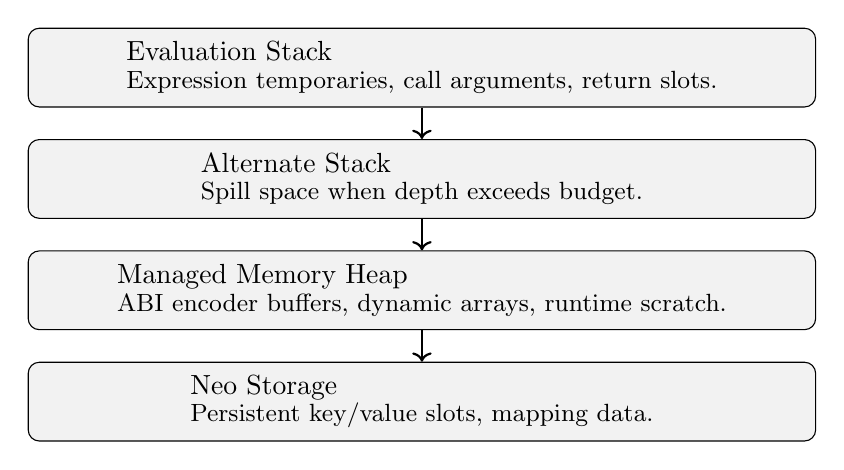
\begin{tikzpicture}[
    block/.style={draw, rounded corners, minimum width=10cm, minimum height=1cm, align=left, fill=gray!10},
    arrow/.style={->, thick}
]
\node[block] (stack) {Evaluation Stack\\[-0.2em]\small Expression temporaries, call arguments, return slots.};
\node[block, below=0.4cm of stack] (altstack) {Alternate Stack\\[-0.2em]\small Spill space when depth exceeds budget.};
\node[block, below=0.4cm of altstack] (mem) {Managed Memory Heap\\[-0.2em]\small ABI encoder buffers, dynamic arrays, runtime scratch.};
\node[block, below=0.4cm of mem] (storage) {Neo Storage\\[-0.2em]\small Persistent key/value slots, mapping data.};
\draw[arrow] (stack) -- (altstack);
\draw[arrow] (altstack) -- (mem);
\draw[arrow] (mem) -- (storage);
\end{tikzpicture}}
\caption{Logical runtime memory layout}
\label{fig:runtime-memory}
\end{figure}

\subsection{Memory Manager Responsibilities}
\begin{itemize}
    \item \textbf{Allocation Model:} Solidity \texttt{memory} allocations map to runtime-managed byte arrays. Each allocation records length and an offset inside a contiguous Neo array; the runtime returns a handle (stack-stored integer) representing the base pointer. \texttt{msize} is implemented by returning the current heap pointer.
    \item \textbf{Load/Store Semantics:} \texttt{mload} reads 32 bytes from the handle's byte array, automatically padding/truncating to the ABI-expected width. \texttt{mstore} writes 32 bytes, while \texttt{mstore8} writes a single byte. Bounds checks are inserted when \texttt{EnableBoundsChecking} is true, causing \texttt{require}-style reverts upon violation.
    \item \textbf{Call Data Buffer:} On entry, the runtime decodes Neo invocation arguments and materializes a calldata buffer in the memory heap. \texttt{calldataload} and \texttt{calldatacopy} operate on this buffer via helper syscalls.
    \item \textbf{Return Data:} ABI encoders reserve memory slices, pack results according to Solidity layout, push (offset, length) pairs on stack, and call the runtime return routine to emit bytes into Neo's VM return channel.
    \item \textbf{Alt Stack Discipline:} Spills occur only when static stack analysis predicts depth \(>\) \texttt{MaxStackDepth}. Spilled values preserve evaluation order by round-tripping through \texttt{TOALTSTACK} / \texttt{FROMALTSTACK} sequences.
\end{itemize}

\subsection{ABI Encoding Rules}
\begin{itemize}
    \item \textbf{Function Selectors:} The dispatcher extracts the first 4 bytes of the invocation data. Neo invocation payloads are expected to match the Solidity ABI layout (selector + encoded args). For Neo-native tooling, CLI wrappers produce compatible payloads.
    \item \textbf{Static Types:} Integers and addresses encode as 32-byte, big-endian values following Solidity conventions; the runtime ensures values stored in Neo's stack (big integers) are normalized before serialization.
    \item \textbf{Dynamic Types:} Arrays and strings encode as (offset, length, data) triples. The runtime writes the data section into contiguous memory, records offsets relative to the ABI root, and ensures padding to 32-byte boundaries.
    \item \textbf{Tuples/Structs:} Flattened according to Solidity rules. Nested dynamic members cause recursive allocation of tail segments with offsets patched once lengths are finalized.
    \item \textbf{Events:} Indexed parameters become topics (handled by \texttt{System.Runtime.Notify}); non-indexed parameters are ABI-encoded in a single byte array passed as the notify payload.
\end{itemize}

\subsection{Error and Panic Translation}
\begin{table}[H]
\centering
\caption{Solidity error mapping}
\begin{tabularx}{\textwidth}{@{}p{0.24\textwidth}p{0.2\textwidth}X@{}}
\toprule
Solidity Construct & Selector & NeoVM Implementation \\
\midrule
\texttt{require(condition, msg)} & \texttt{0x08c379a0} & Condition lowered to predicate; on failure, encode string reason via ABI encoder, call shared revert stub that writes selector + data to return buffer and halts execution.\\
\texttt{assert(condition)} & \texttt{0x4e487b71} (panic) & On failure, emit panic code (per Solidity spec) and revert. Panic codes stored as constants in codegen, ensuring deterministic mapping.\\
\texttt{revert CustomError(args)} & \texttt{keccak("Error(...")} & Lowered to runtime call that writes custom selector + encoded args.\\
\texttt{invalid} opcode & none & Raises immediate VM fault; compiler only emits for unrecoverable states or unreachable detection.\\
\bottomrule
\end{tabularx}
\end{table}

\subsection{Runtime Logging and Instrumentation}
\begin{itemize}
    \item \textbf{Structured Logs:} The compiler injects logging stubs (guarded by a configuration flag) that emit structured events via \texttt{System.Runtime.Trace} for critical transitions (dispatcher entry, storage writes, external calls). These logs aid debugging without impacting release builds when disabled.
    \item \textbf{Execution Tracing:} An optional tracing mode wraps each function entry/exit with \texttt{TRACE} events carrying method names and offsets. This mode uses metadata from \texttt{FunctionInfo} to keep logs human-readable.
    \item \textbf{Error Channels:} Revert helpers push error selectors and encoded payloads into the return buffer and also log the selector + message via \texttt{System.Runtime.Log}, enabling node operators to correlate on-chain failures with runtime logs.
    \item \textbf{Instrumentation Hooks:} The runtime exposes hooks that the CLI can enable, such as stack depth counters and syscall counters. These feed into \texttt{CompilationStats} and optional telemetry outputs for optimizer tuning.
\end{itemize}

\paragraph{Logging Pseudocode}
\begin{verbatim}
procedure guarded_storage_put(slot, value):
    if logging_enabled:
        SYSCALL System.Runtime.Trace("StoragePut", slot, value)
    SYSCALL System.Storage.PutContext(slot, value)
\end{verbatim}

\section{Debug Information and Diagnostics}
\subsection{Debug Artifact Structure}
\begin{table}[H]
\centering
\caption{\texttt{nef.debug.json} fields}
\begin{tabularx}{\textwidth}{@{}p{0.22\textwidth}p{0.2\textwidth}X@{}}
\toprule
Field & Type & Description \\
\midrule
\texttt{sourceMap} & array & Entries mapping bytecode offset \(\rightarrow\) source file, line, column. Derived from \texttt{buildSourceMap}.\\
\texttt{functions} & array & Function info objects (name, offset range, parameter metadata, local variable descriptors). Mirrors \texttt{FunctionInfo}.\\
\texttt{locals} & array & Variable table entries referencing stack slot numbers or storage locations; used by debugger to show state.\\
\texttt{sequencePoints} & array & Per-instruction mapping enabling step-into/step-over semantics.\\
\texttt{contracts} & object & Summary of compiled contracts, metadata, and manifest hash for traceability.\\
\bottomrule
\end{tabularx}
\end{table}

\subsection{Diagnostic Life Cycle}
\begin{enumerate}
    \item \textbf{Collection:} Each stage populates \texttt{ErrorCollector}. Diagnostics include phase, severity, message, source span, and machine-readable identifiers for tooling integration.
    \item \textbf{Emission Ordering:} Diagnostics are sorted by file, then line, ensuring stable output. CLI tooling can render them in IDE-friendly formats (JSON, plain text).
    \item \textbf{Stage Gates:} Parsing and normalization errors halt compilation immediately; semantic errors block optimization/codegen; runtime integration errors occur only after code generation. Warnings propagate but do not halt unless \texttt{--fail-on-warning} is passed.
    \item \textbf{External Reporting:} Batch compilation routines (e.g., Uniswap suite) log per-file status in \path{compile_summary.csv}, capturing counts of errors/warnings for CI dashboards.
    \item \textbf{Debug Synchronization:} When \texttt{EnableDebugInfo} is true, source/diagnostic metadata embed build identifiers so IDE sessions can ensure the debug artifact matches the loaded NEF.
\end{enumerate}

\subsection{Debugger Interaction Flow}
\begin{enumerate}
    \item IDE loads NEF and associated \texttt{nef.debug.json}.
    \item Breakpoints are set using source positions; IDE uses \texttt{sourceMap} to translate into bytecode offsets.
    \item During execution, Neo debugger emits instruction offsets; tooling maps offsets back to source using \texttt{sequencePoints} and displays live stack/locals using \texttt{locals} metadata.
    \item Variable inspection relies on stack location metadata (slot indices) or storage offsets computed during semantic analysis. For mappings, debugger uses the recorded hashing recipe to fetch storage entries.
    \item When stepping out, debugger consults \texttt{functions} offsets to jump to caller location, guaranteeing consistent view with the compiled ABI.
\end{enumerate}

\section{Illustrative Example}
\subsection{Sample Solidity Fragment}
\begin{verbatim}
function transfer(address to, uint256 amount) external returns (bool) {
    require(balances[msg.sender] >= amount, "insufficient");
    balances[msg.sender] -= amount;
    balances[to] += amount;
    emit Transfer(msg.sender, to, amount);
    return true;
}
\end{verbatim}

\subsection{Canonical Yul Form (Excerpt)}
\begin{verbatim}
function transfer(to, amount) -> success {
    let sender := caller()
    let slot := balances_slot
    let sender_slot := mapping_slot(slot, sender)
    let sender_balance := sload(sender_slot)
    if lt(sender_balance, amount) {
        revert_insufficient()
    }
    sstore(sender_slot, sub(sender_balance, amount))
    let to_slot := mapping_slot(slot, to)
    sstore(to_slot, add(sload(to_slot), amount))
    logTransfer(sender, to, amount)
    success := 1
}
\end{verbatim}

\subsection{NeoVM Emission Trace (Key Instructions)}
\begin{longtable}{@{}p{0.14\textwidth}p{0.27\textwidth}p{0.45\textwidth}@{}}
\caption{Transfer lowering trace}\\
\toprule
IR Step & Stack Input & NeoVM Sequence \\
\midrule
\endfirsthead
\toprule
IR Step & Stack Input & NeoVM Sequence \\
\midrule
\endhead
Load caller & -- & \texttt{SYSCALL System.Runtime.GetCallingScriptHash} (runtime maps to EVM caller).\\
Mapping slot (sender) & \([sender]\) & Call \texttt{emit\_mapping\_slot(slot\_hash, [sender])}. See Section~\ref{sec:mapping-detail}.\\
Balance load & \([slot]\) & \texttt{System.Storage.GetContext}; \texttt{SWAP}; \texttt{SYSCALL System.Storage.Get}.\\
Require check & \([balance, amount]\) & \texttt{DUP2}; \texttt{LT}; \texttt{JMPIF revert\_label}.\\
Subtract amount & \([balance, amount]\) & \texttt{SUB}; push slot; reorder; \texttt{System.Storage.Put}.\\
Increment recipient & \([recipient]\) & Repeat mapping slot derivation, load existing balance, \texttt{ADD}, store via \texttt{System.Storage.Put}.\\
Emit event & \([sender, to, amount]\) & ABI-encode topic/data arrays, call \texttt{System.Runtime.Notify}.\\
Return true & -- & \texttt{PUSH1}; ABI encode boolean return; \texttt{RET}.\\
\bottomrule
\end{longtable}

\subsection{NEF and Manifest Excerpts}
\paragraph{Method Token (pseudo)}
\begin{verbatim}
{
  "name": "transfer",
  "parameters": 2,
  "return": 1,
  "offset": 0x0234
}
\end{verbatim}

\paragraph{Manifest Snippet}
\begin{verbatim}
"abi": {
  "methods": [
    {
      "name": "transfer",
      "offset": "0x0234",
      "parameters": [
        {"name": "to", "type": "Hash160"},
        {"name": "amount", "type": "Integer"}
      ],
      "returntype": "Boolean",
      "safe": false
    }
  ],
  "events": [
    {
      "name": "Transfer",
      "parameters": [
        {"name": "from", "type": "Hash160", "indexed": true},
        {"name": "to", "type": "Hash160", "indexed": true},
        {"name": "amount", "type": "Integer", "indexed": false}
      ]
    }
  ]
},
"permissions": [
  {"contract": "0x0", "methods": ["System.Runtime.Notify", "System.Storage.*"]}
],
"supportedstandards": ["NEP-17"]
\end{verbatim}

\subsection{End-to-End Trace Notes}
\begin{itemize}
    \item The require string ``insufficient'' is interned once in a read-only data section, referenced by the revert helper when encoding the ABI payload.
    \item Debug info associates the \texttt{transfer} function body with bytecode offsets \(0x0234\)–\(0x03EF\); breakpoints set in Solidity source map to these offsets using \texttt{sequencePoints}.
    \item Gas accounting records two storage reads + two writes, one event emission, and constant arithmetic operations; these metrics feed the manifest's optional \texttt{extra} metadata for auditing.
\end{itemize}
\subsection{Manifest JSON Example}
\begin{small}
\begin{verbatim}
{
  "name": "SampleToken",
  "groups": [],
  "supportedstandards": ["NEP-17"],
  "abi": {
    "methods": [
      {
        "name": "transfer",
        "parameters": [
          {"name": "to", "type": "Hash160"},
          {"name": "amount", "type": "Integer"}
        ],
        "returntype": "Boolean",
        "offset": "0x0234",
        "safe": false
      }
    ],
    "events": [
      {
        "name": "Transfer",
        "parameters": [
          {"name": "from", "type": "Hash160", "indexed": true},
          {"name": "to", "type": "Hash160", "indexed": true},
          {"name": "amount", "type": "Integer", "indexed": false}
        ]
      }
    ]
  },
  "permissions": [
    {"contract": "0x0000...0000", "methods": ["System.Storage.*"]},
    {"contract": "0x0000...0000", "methods": ["System.Runtime.Notify"]}
  ],
  "features": {
    "storage": true,
    "dynamicInvoke": false,
    "payable": false
  },
  "extra": {
    "compilerVersion": "neo-solidity 1.0.0",
    "optimizationLevel": "O2",
    "sourceHash": "0x..."
  }
}
\end{verbatim}
\end{small}
\subsection{Debug JSON Excerpt}
\begin{small}
\begin{verbatim}
{
  "sourceMap": [
    {"offset": 0x0234, "file": "Token.sol", "line": 10, "column": 4},
    {"offset": 0x0241, "file": "Token.sol", "line": 11, "column": 8}
  ],
  "functions": [
    {"name": "transfer", "start": 0x0234, "end": 0x03ef, "params": 2, "returns": 1}
  ],
  "locals": [
    {"function": "transfer", "name": "sender", "storage": "stack", "slot": 2},
    {"function": "transfer", "name": "amount", "storage": "stack", "slot": 0}
  ],
  "sequencePoints": [
    {"offset": 0x0234, "document": "Token.sol", "line": 10},
    {"offset": 0x0270, "document": "Token.sol", "line": 14}
  ],
  "contracts": [
    {"name": "SampleToken", "manifestHash": "0x...", "sourceHash": "0x..."}
  ]
}
\end{verbatim}
\end{small}
\subsection{Method Token Table}
\begin{table}[H]
\centering
\caption{Example method tokens}
\begin{tabularx}{\textwidth}{@{}p{0.25\textwidth}p{0.15\textwidth}p{0.15\textwidth}X@{}}
\toprule
Method & Offset & Parameters & Notes \\
\midrule
\texttt{_deploy} & \(0x0000\) & 1 & Constructor entry; invoked once at deployment with data payload.\\
\texttt{transfer} & \(0x0234\) & 2 & External ABI entry; safe flag determined by analyzer.\\
\texttt{balanceOf} & \(0x0350\) & 1 & View method; safe flag set to true as no storage writes occur.\\
\texttt{_main} & \(0x0400\) & 0 & Dispatcher that routes based on ABI selector.\\
\bottomrule
\end{tabularx}
\end{table}
\subsection{Runtime Lookup of Debug Metadata}
\begin{itemize}
    \item \textbf{Offset Tables:} During compilation, \texttt{InstructionInfo} entries reference the owning method token. Runtime tooling uses this mapping to resolve which function a given offset belongs to, enabling quick lookups without scanning the entire debug JSON.
    \item \textbf{Source Hash Guards:} Both manifest \texttt{extra.sourceHash} and debug JSON \texttt{contracts[*].sourceHash} store the same digest recorded in \texttt{CompilationMetadata}. Debuggers verify equality before trusting source/offset mappings to avoid stale metadata.
    \item \textbf{Storage Slot Reconstruction:} For state variables, the debug JSON carries either direct slot identifiers (for flat variables) or a reference to the hashing recipe defined in Section~\ref{sec:mapping-detail}. Tooling reproduces the hashing steps when inspecting mappings during a paused execution.
    \item \textbf{Scope Hierarchy:} Functions and locals reference parent scopes so IDEs can draw call stacks and inspect nested blocks. Each scope entry lists its active stack slots and captured storage references, allowing accurate watch window display even during inlined code.
\end{itemize}
\subsection{Build and Deployment Workflow}
\begin{enumerate}
    \item \textbf{Build Compiler Binaries:} Run \texttt{cargo build --release} to produce the Rust-based CLI and Go components, ensuring environment matches README prerequisites (Rust 1.70+, dotnet runtime for devpack).
    \item \textbf{Compile Contracts:} Invoke \texttt{target/release/neo-solc Contract.sol -O2 -o build/Contract} to emit \path{Contract.nef} and \path{Contract.manifest.json}. Batch mode uses the pipeline shown in README (e.g., \texttt{find ... | xargs neo-solc}).
    \item \textbf{Validate Outputs:} Run \texttt{neo-cli contract deploy} against the NEF + manifest to verify the contract executes as expected on Neo N3 TestNet. Manifest permissions should match the emitted syscalls; mismatches cause deployment rejections.
    \item \textbf{CI Packaging:} On successful builds, CI uploads NEF/manifest artifacts, \path{compile_summary.csv}, and \path{spec/neo_solidity_compiler_design_spec.pdf} for traceability. Release tags trigger binary packaging for multiple platforms.
\end{enumerate}

\subsection{Release Process}
\begin{enumerate}
    \item \textbf{Versioning:} Update \texttt{Cargo.toml}, Go module metadata, and the spec title if a major/minor release occurs. Follow semantic versioning aligned with Neo N3 support milestones.
    \item \textbf{Tagging:} Create a signed git tag (e.g., \texttt{v1.0.0}) once the CI pipeline passes. Tag creation triggers the release workflow that bundles binaries and documentation.
    \item \textbf{Artifact Bundling:} Run \texttt{scripts/package_release.sh}, producing platform-specific binaries (\texttt{neo-solc-linux}, \texttt{neo-solc-macos}, etc.), sample NEFs/manifests, and the PDF spec. Attach these artifacts to the GitHub release along with checksums.
    \item \textbf{Documentation Sync:} Ensure README, CHANGELOG, and the LaTeX spec reflect the release state. The release workflow uploads \path{spec/neo_solidity_compiler_design_spec.pdf} alongside binaries so consumers have the authoritative design reference.
    \item \textbf{Post-Release Validation:} Deploy sample contracts using the released binary on TestNet/MainNet, verifying manifests, events, and ExecutionOverrides behavior match expectations. Document any known issues for the next milestone.
\end{enumerate}

\subsection{Release Summary}
\begin{itemize}
    \item \textbf{Artifacts:} Each release ships platform-specific \texttt{neo-solc} binaries, reference NEF/manifest pairs, compile summaries, metrics reports, and the updated PDF spec.
    \item \textbf{Documentation Sync:} README, CHANGELOG, and tooling docs link to the release-specific spec. Hardhat/Foundry integration guides reference the matching compiler version.
    \item \textbf{Verification:} Releases are tested on Neo TestNet/MainNet using canonical contracts; results (transaction IDs, manifest hashes) are noted in release notes for reproducibility.
    \item \textbf{Support Window:} The team maintains at least the latest release and the previous minor version, backporting fixes for security issues when necessary.
\end{itemize}

\subsection{CLI Interface Reference}
\begin{table}[H]
\centering
\caption{\texttt{neo-solc} key options}
\begin{tabularx}{\textwidth}{@{}p{0.22\textwidth}p{0.15\textwidth}X@{}}
\toprule
Flag & Default & Description \\
\midrule
\texttt{-O\{0-3\}} & \texttt{-O2} & Selects optimization pipeline (none through aggressive); maps to \texttt{CompilerConfig.OptimizationLevel}.\\
\texttt{--debug} & \texttt{false} & Emits \texttt{nef.debug.json} and populates \texttt{CompilationResult.DebugInfo}.\\
\texttt{--source-map} & \texttt{false} & Forces source map generation even when debug bundle disabled.\\
\texttt{-f \<formats\>} & \texttt{nef,manifest} & Chooses output formats (e.g., \texttt{-f nef} or \texttt{-f manifest,abi}).\\
\texttt{-o \<path\>} & current dir & Destination path prefix for NEF/manifest outputs.\\
\texttt{--target-neovm \<version\>} & detected & Overrides target NeoVM version for syscall gating and manifest metadata.\\
\texttt{--manifest-only} & \texttt{false} & Rewrites manifest based on cached IR/metadata without regenerating NEF.\\
\texttt{--fail-on-warning} & \texttt{false} & Treats compiler warnings as errors, stopping the pipeline earlier.\\
\texttt{--emit-ir} & \texttt{false} & Dumps canonical IR (Yul-normalized) for debugging optimization pipelines.\\
\bottomrule
\end{tabularx}
\end{table}

\subsection{Developer Workflow Checklist}
\begin{enumerate}
    \item \textbf{Environment Setup:} Install Rust 1.70+, Go toolchain, dotnet runtime (for devpack), and Neo CLI for deployment validation.
    \item \textbf{Lint \& Format:} Run \texttt{cargo fmt}, \texttt{cargo clippy}, Go formatters, and TypeScript linters (for tooling packages). Lint failure blocks PR merges.
    \item \textbf{Unit Tests:} Execute \texttt{cargo test --all} and relevant Go tests to catch regressions in lexers, parsers, codegen helpers.
    \item \textbf{Integration Tests:} Compile the NEP suite and Uniswap set; inspect \path{compile_summary.csv} for deterministic success. Failures require root-cause notes before merging.
    \item \textbf{Manual Verification (as needed):} Deploy representative NEF/manifest outputs onto Neo TestNet via \texttt{neo-cli} or NeoExpress to validate runtime behavior.
    \item \textbf{Documentation Update:} When behavior changes, regenerate \path{spec/neo_solidity_compiler_design_spec.pdf} to keep the formal spec aligned with implementation.
\end{enumerate}
